\documentclass[10pt]{article}
\usepackage{icmlko}

\icmlmeta{IP 파운데이션 월드모델}{344}{머리카락 한 올}{검사 ① 을 0.004 차로 떨어진 축이 검사 ⑤ 를 통과했다 --- 채택은 하되 문턱은 안 옮긴다}

\begin{document}

\twocolumn[
\icmlheader

\begin{abstract}
노트 343의 여섯 번째 목록(\texttt{tagaxes.FIELDS} 대 \texttt{SPEC})을
도구로 훑었다. \textbf{후보가 셋 더 나온다} --- 만화 \texttt{genres}
16종(학습 1,783) · 세계애니 18종(2,648) · 게임 9종(259). 셋 다
\texttt{FIELDS} 에도 \texttt{SPEC} 에도 없었다.

\textbf{검사 ①②③ 이 셋을 다 걸렀다.} 만화는 ①②(제일 센 성분이 $\rho$
$+$0.121 에 조각 4/5), 게임은 ③(겹침 0.449 --- \texttt{goods\_scale} 의
흐린 사본), \textbf{세계애니는 ① 을 0.004 차로}($\rho$ $+$0.116 · 문턱
0.12).

\textbf{그래서 떨어진 둘에 검사 ⑤ 를 돌렸다} --- 문턱이 제자리인지
새 도구로 보려는 것이다.

\begin{center}\footnotesize
\begin{tabular}{llrr}
\hline
후보 & 왜 떨어졌나 & 검사 ⑤ 판 & 양수 \\
\hline
\textbf{세계애니} & ① 0.116 & \textbf{$+$0.0027} & \textbf{7/8} \\
게임 & ③ 0.449 & $-$0.0004 & 5/8 \\
\hline
\end{tabular}
\end{center}

\textbf{③ 은 옳게 걸렀고 ① 은 잘못 걸렀다.} 겹침으로 떨어진 게임 장르는
제 쌍둥이도 못 이기는데, 상관 문턱을 머리카락 한 올 차로 못 넘은 세계애니
장르는 제 도메인에서 8/8 로 이긴다($+$0.0105).

\textbf{붙였다} --- 세계애니 $+$0.0063(SD 0.0034 · \textbf{12/12}) ·
판 $+$0.0015(SD 0.0025 · 8/12). 배포 규칙 ①② 통과. \textbf{채택한다.}

\textbf{그런데 문턱은 안 옮긴다.} 0.12 를 0.11 로 내리면 \emph{이 하나로}
법칙을 세우는 것이고, 노트 342가 방금 ``n$=$1 로 세운 법칙은 n$=$4 를 못
견딘다''를 배웠다. \textbf{채택은 검사 ⑤ 와 배포 규칙으로 하고, 문턱은
후보가 더 모이면 따로 잰다.}
\end{abstract}
]

\section{훑기}

\begin{center}\footnotesize
\begin{tabular}{lrrl}
\hline
도메인 & 학습 & 토큰 & 상태 \\
\hline
웹툰 & 2,106 & 121 & 축 있음 \\
애니 & 1,467 & 122 & 축 있음 \\
모바일 & 1,559 & 46 & \textbf{노트 343에서 채택} \\
만화 & 1,783 & 16 & ①② 탈락 \\
\textbf{세계애니} & 2,648 & 18 & \textbf{오늘 채택} \\
게임 & 259 & 9 & ③ 탈락 \\
도서 · 펀딩 & --- & 0 & 토큰 없음 \\
\hline
\end{tabular}
\end{center}

\begin{figure*}[t]
\centering
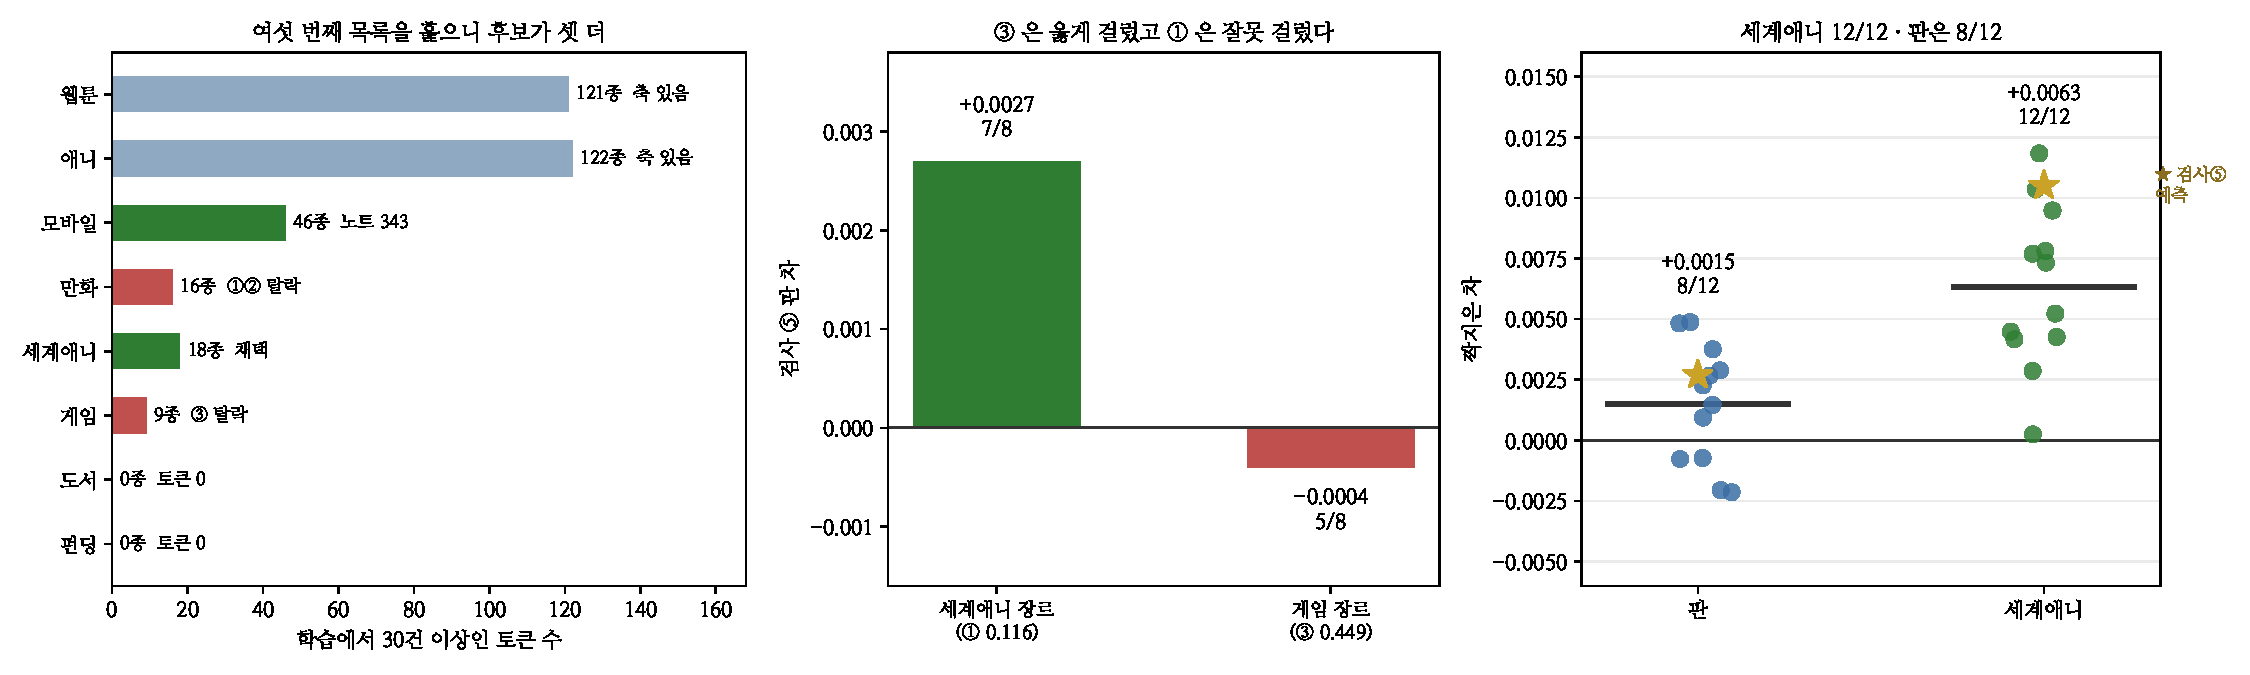
\includegraphics[width=\textwidth]{figs/hair.pdf}
\caption{왼쪽 --- 훑기. 가운데 --- 떨어진 둘에 검사 ⑤. 오른쪽 --- 붙인 결과.}
\end{figure*}

\section{③ 은 옳고 ① 은 아깝다}

\begin{center}\footnotesize
\begin{tabular}{lrrrl}
\hline
후보 & $\rho$ & 조각 & 겹침 & 검사 ⑤ \\
\hline
세계애니 성분 2 & $+$0.116 & 5/5 & 0.174 & \textbf{$+$0.0027 (7/8)} \\
세계애니 성분 3 & $-$0.110 & 5/5 & 0.132 & \\
게임 성분 0 & $-$0.174 & 5/5 & \textbf{0.449} & $-$0.0004 (5/8) \\
\hline
\end{tabular}
\end{center}

게임 성분 0 에 실린 토큰이 \texttt{g:액션} $-$0.61 · \texttt{g:시뮬레이션}
$+$0.52 인데 \texttt{goods\_scale} 과 0.449 다 --- 노트 256이 ``흐린
사본이 나무를 깨뜨린다''고 만든 문턱이고, \textbf{검사 ⑤ 가 같은 판정을
낸다.} 두 검사가 독립적으로 맞았다.

세계애니 성분 2 는 \texttt{g:Action} $-$0.56 · \texttt{g:Slice of Life}
$+$0.41 로 장르 대비이고 겹침이 0.174 다. \textbf{①만 0.004 모자랐다.}

\section{붙였다}

\begin{center}\footnotesize
\begin{tabular}{lrrr}
\hline
 & 평균 & SD & 양수 \\
\hline
\textbf{세계애니} & \textbf{$+$0.0063} & 0.0034 & \textbf{12/12} \\
도서 & $+$0.0107 & 0.0235 & 6/12 \\
게임 & $+$0.0033 & 0.0051 & 9/12 \\
팝업 & $-$0.0073 & 0.0147 & 3/12 \\
펀딩 & $-$0.0058 & 0.0104 & 3/12 \\
\hline
\textbf{판} & $+$0.0015 & 0.0025 & 8/12 \\
\hline
\end{tabular}
\end{center}

\textbf{제 도메인은 12/12 로 확실하고 판은 8/12 로 못 가른다.} 세계애니가
판의 11\%라 $+$0.0063 이 판에 $+$0.0007 만 실린다 --- 나머지는 남의
움직임이다. 배포 규칙은 통과한다(제일 나쁜 도메인 팝업 $-$0.0073 ·
짝SE 0.045 · $t{\approx}0.16$).

\paragraph{검사 ⑤ 의 정확도} 노트 343에서는 판 $+$0.0042 예측에 실제
$+$0.0041 이었다. 오늘은 $+$0.0027 예측에 $+$0.0015 --- \textbf{방향은
맞고 크기는 60\%다.} 두 사례로는 ``얼마나 정확한가''를 못 말한다.

\section{문턱은 안 옮긴다}

\begin{center}\small
\begin{tabular}{ll}
\hline
채택 근거 & 검사 ②③⑤ $+$ 배포 규칙 \\
안 하는 것 & 검사 ① 문턱 0.12 $\to$ 0.11 \\
왜 & \textbf{후보가 하나다} \\
\hline
\end{tabular}
\end{center}

노트 342가 ``n$=$1 로 세운 법칙은 n$=$4 를 못 견딘다''를 겪었다. 문턱을
옮기는 것은 앞으로 모든 후보에 적용되는 법칙이고, \textbf{그것을 세우려면
0.10$\sim$0.12 구간의 후보가 여럿 필요하다.} 오늘은 축 하나를 채택할
뿐이다.

\section{남은 것}
\begin{center}\footnotesize
\begin{tabular}{ll}
\hline
갈래 & 왜 \\
\hline
\textbf{① 문턱 구간의 후보 모으기} & 0.10$\sim$0.12 짜리를 여럿 \\
검사 ⑤ 의 정확도 & 두 사례로는 못 말한다 \\
만화 장르를 다시 & 조각 4/5 --- ② 가 진짜 문제인가 \\
팝업 · 펀딩이 왜 지나 & 남의 축인데 내려간다 \\
\hline
\end{tabular}
\end{center}

\paragraph{규약} \textbf{한 후보를 채택하는 것과 문턱을 옮기는 것은 다른
결정이다.} 오늘 세계애니 장르가 검사 ① 을 0.004 차로 못 넘고 검사 ⑤ 를
통과했다. 그 둘을 한 번에 처리하고 싶은 유혹이 있다 --- ``문턱이 틀렸으니
내리고 붙이자.'' \textbf{그러면 하나의 관측으로 앞으로의 모든 판정을
바꾸는 것이다.} 채택은 되돌릴 수 있고 문턱은 잘 안 되돌아온다.
\textbf{되돌리기 쉬운 쪽부터 한다.}

\end{document}
